% =============================================================================
% Adaptive Frame Processing: Latency-Bounded Temporal Scheduling
% for Multi-Modal Edge Inference
% IEEE Conference Format — Track 6: Signal Processing, Computing & Data Science
% =============================================================================
\documentclass[conference]{IEEEtran}
\IEEEoverridecommandlockouts

\usepackage{cite}
\usepackage{amsmath,amssymb,amsfonts}
\usepackage{algorithmic}
\usepackage{algorithm}
\usepackage{graphicx}
\usepackage{textcomp}
\usepackage{xcolor}
\usepackage{booktabs}
\usepackage{tikz}
\usetikzlibrary{arrows.meta, positioning, shapes.geometric, calc}
\usepackage{balance}

\def\BibTeX{{\rm B\kern-.05em{\sc i\kern-.025em b}\kern-.08em
    T\kern-.1667em\lower.7ex\hbox{E}\kern-.125emX}}

% =============================================================================
% SPACE-SAVING ADJUSTMENTS (Strictly IEEEtran template compliant)
% =============================================================================
\setlength{\textfloatsep}{8pt plus 2.0pt minus 2.0pt}
\setlength{\floatsep}{8pt plus 2.0pt minus 2.0pt}
\setlength{\intextsep}{8pt plus 2.0pt minus 2.0pt}
\setlength{\dbltextfloatsep}{8pt plus 2.0pt minus 2.0pt}
\setlength{\dblfloatsep}{8pt plus 2.0pt minus 2.0pt}
\def\IEEEbibitemsep{0pt plus 1.0pt}

\begin{document}

% =============================================================================
% TITLE AND AUTHORS
% =============================================================================
\title{Adaptive Frame Processing: Latency-Bounded\\
Temporal Scheduling for Multi-Modal Edge Inference}

\author{
  \IEEEauthorblockN{Anonymous Authors}
  \IEEEauthorblockA{
    \textit{Anonymous Affiliation} \\
    Anonymous City, Anonymous Country \\
    anonymous@example.com
  }
}

\maketitle

% =============================================================================
% ABSTRACT
% =============================================================================
\begin{abstract}
Real-time multi-modal video inference on edge CPUs must execute
depth estimation and object detection under tight compute budgets.
Static frame subsampling reduces average load but imposes fixed
worst-case response delays regardless of scene content. We present
Adaptive Frame Processing (AFP), a temporal scheduling framework
that adjusts per-frame processing rates via a one-frame depth
feedback loop, concentrating compute on proximity-critical frames
while skipping redundant content. AFP resolves the circular
dependency between scheduling decisions and depth computation
without auxiliary policy networks. On 24 real-world video sequences
(7,683 frames) with CPU-only ONNX inference, AFP achieves an
87.6\% frame skip ratio with detection coverage matching static
1/10 subsampling (TOST equivalence, $p < 0.001$,
$\delta{=}{\pm}5$\,pp), while
bounding worst-case proximity response latency at 200\,ms compared
to 900\,ms for static and unbounded latency for motion-triggered
baselines. The amortized per-frame cost is 10.8\,ms on a consumer
CPU.
\end{abstract}

\begin{IEEEkeywords}
temporal scheduling, adaptive computation, edge inference,
depth estimation, object detection, video processing
\end{IEEEkeywords}

% =============================================================================
% I. INTRODUCTION
% =============================================================================
\section{Introduction}
\label{sec:introduction}

Deploying multi-modal video perception on edge
devices---autonomous robots, IoT monitoring platforms, mobile
systems---requires running multiple deep neural networks per frame.
A representative pipeline combining monocular depth
estimation~\cite{ranftl2020midas} with object
detection~\cite{jocher2023yolov8} takes approximately 87\,ms per
frame on a consumer-grade CPU, saturating the real-time budget at
modest frame rates. Model-level optimizations such as
quantization~\cite{jacob2018quantization} and lightweight
architectures~\cite{howard2017mobilenets} reduce per-inference cost
but leave a major source of inefficiency untouched: temporal
redundancy in video streams.

Static subsampling---processing every $N$th frame and returning
cached results otherwise---exploits this redundancy at the cost of
a fixed worst-case response delay of $(N{-}1)/f$ seconds, where $f$
is the frame rate. At $N{=}10$ and $f{=}10$\,fps, the system takes
up to 900\,ms to react to a new event regardless of scene dynamics.
Motion-triggered approaches process frames only when inter-frame
change exceeds a threshold. These adapt to scene activity but fail
when scenes change slowly or hazards are static, causing the trigger
threshold to never be reached and the response latency to grow
without bound.

We present \emph{Adaptive Frame Processing} (AFP), a temporal
scheduling framework that adjusts frame processing rates based on
scene content. AFP uses two signals from the prior inference cycle:
(i)~a proximity signal derived from the monocular depth map, and
(ii)~a stability signal from histogram correlation. When objects are
close, AFP increases processing frequency to bound response latency;
when scenes are stable and distant, it skips aggressively.
The core novelty of AFP lies in resolving a fundamental circular
dependency: the optimal temporal scheduling decision depends on
depth information, but computing depth is the exact operation being
scheduled. AFP's one-frame depth-feedback loop resolves this
dependency. By doing so, it provides formal latency-bounded
scheduling guarantees without the complexity of training an
auxiliary policy network.

This paper makes three contributions:
\begin{enumerate}
  \item A temporal scheduling framework for multi-modal edge
    inference that uses depth feedback to dynamically adjust frame
    skip rates, resolving the circular scheduling dependency without
    learned policy models.
  \item A formal analysis of worst-case response latency under
    static, motion-triggered, and adaptive scheduling, showing that
    AFP bounds proximity latency at 200\,ms while static 1/10
    incurs 900\,ms and motion-triggered approaches are unbounded.
  \item An empirical evaluation on 24 real-world video sequences
    (7,683 frames) showing that AFP achieves 87.6\% frame skip with
    detection coverage statistically equivalent to static
    subsampling (TOST equivalence, $p < 0.001$,
    $\delta{=}{\pm}5$\,pp).
\end{enumerate}

All experiments use CPU-only inference via ONNX
Runtime~\cite{onnxruntime2019} on a consumer processor, with no GPU
or accelerator dependencies.

The remainder of this paper is organized as follows.
Section~\ref{sec:related} reviews related work.
Section~\ref{sec:pipeline} describes the inference pipeline.
Section~\ref{sec:afp} presents the AFP framework and its latency
bounds. Section~\ref{sec:experiments} evaluates AFP against multiple
baselines on real-world data, and Section~\ref{sec:conclusion}
concludes.

% =============================================================================
% II. RELATED WORK
% =============================================================================
\section{Related Work}
\label{sec:related}

\subsection{Within-Frame Adaptive Computation}

Several methods adapt computational effort to input complexity
within a single forward pass.
BlockDrop~\cite{wu2018blockdrop} learns to skip residual blocks per
image. SkipNet~\cite{wang2018skipnet} routes inputs through
dynamically selected layers.
BranchyNet~\cite{teerapittayanon2016branchynet} introduces early
exits, and Figurnov et al.~\cite{figurnov2017spatially} proposed
spatially adaptive computation time for residual networks. These
approaches reduce per-frame model cost. AFP is complementary: it
operates \emph{across} frames, adjusting the temporal processing
rate based on scene context.

\subsection{Across-Frame Adaptive Inference}

Content-dependent frame selection is a well-studied area.
AdaFrame~\cite{wu2019adaframe} and
FrameExit~\cite{ghodrati2021frameexit} use reinforcement learning
to decide which frames to process.
SCSampler~\cite{korbar2019scsampler} and
OCSampler~\cite{xie2021ocsampler} select salient clips for
efficient video recognition.
SMART~\cite{smart2020smart} performs adaptive multi-task frame
sampling. AR-Net~\cite{meng2020arnet} dynamically adjusts frame
resolution, LiteEval~\cite{qi2019liteeval} employs coarse-to-fine
model selection, AdaFuse~\cite{han2021adafuse} adaptively fuses
temporal features, and
Skip-Convolutions~\cite{habibian2021skip} reuse computations across
similar frames. AFP differs from these methods in two respects.
First, it targets real-time streaming inference on edge CPUs rather
than offline video classification, where worst-case latency matters
more than average accuracy. Second, unlike RL-based or learned policies
that require extensive per-environment training, AFP uses a lightweight,
training-free depth-feedback heuristic. This allows zero-shot deployment
with negligible scheduling overhead (2.6\,ms). Given these deployment constraints, we benchmark AFP against static and motion-triggered baselines rather than learning-based methods.

\subsection{Efficient Edge Deployment}

MobileNets~\cite{howard2017mobilenets} and
EfficientNet~\cite{tan2019efficientnet} reduce model complexity via
depthwise separable convolutions and compound scaling.
Quantization~\cite{jacob2018quantization} and knowledge
distillation~\cite{hinton2015distilling} further compress models for
constrained hardware. ONNX Runtime~\cite{onnxruntime2019} provides
cross-platform inference with CPU-optimized graph transformations.
These optimizations operate at the model level. AFP is orthogonal:
even the most efficient model wastes computation when applied to
temporally redundant frames.

% =============================================================================
% III. INFERENCE PIPELINE
% =============================================================================
\section{Inference Pipeline}
\label{sec:pipeline}

Fig.~\ref{fig:architecture} shows the pipeline architecture. Video
frames enter the AFP scheduler, which decides whether to process or
skip each frame based on the prior frame's depth map and scene
stability. Processed frames pass through two ONNX models executed
sequentially on CPU. MiDaS-Small~\cite{ranftl2020midas} (63.7\,MB)
estimates a relative monocular depth map in 22.8\,ms (median).
YOLOv8-Nano~\cite{jocher2023yolov8} (12.3\,MB) detects objects in
30.0\,ms. For each detection bounding box $(x_1, y_1, x_2, y_2)$,
the median depth value within that region provides a proximity
estimate. The combined pipeline processes a frame in 87.4\,ms, with
depth--detection fusion adding 2.6\,ms overhead (3.0\%). Skipped
frames return cached results at negligible cost
($<$0.01\,ms). Table~\ref{tab:models} summarizes model
characteristics.

\begin{figure}[t]
  \centering
  \resizebox{\columnwidth}{!}{%
  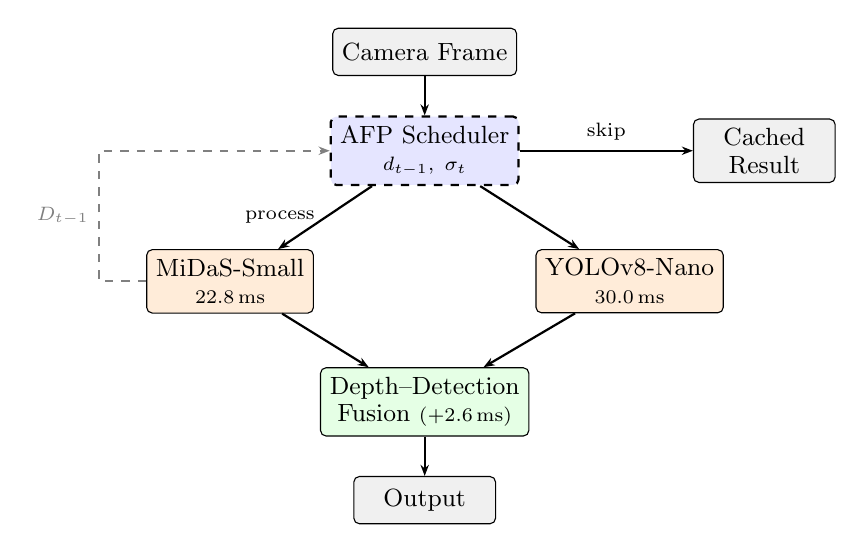
\begin{tikzpicture}[
    box/.style={rectangle, draw, rounded corners=2pt,
                minimum width=1.8cm, minimum height=0.6cm,
                align=center, font=\small},
    model/.style={box, fill=orange!15},
    afp/.style={box, fill=blue!10, thick, dashed},
    io/.style={box, fill=gray!12},
    proc/.style={box, fill=green!10},
    arr/.style={-{Stealth[length=4pt]}, thick},
  ]
    % Input
    \node[io] (cam) {Camera Frame};

    % AFP scheduler
    \node[afp, below=0.5cm of cam] (afp)
      {AFP Scheduler\\[-1pt]
       \scriptsize$d_{t-1},\;\sigma_t$};

    % Skip path
    \node[io, right=2.2cm of afp] (cache) {Cached\\[-1pt]Result};

    % Models
    \node[model, below left=0.8cm and 0.2cm of afp] (midas)
      {MiDaS-Small\\[-1pt]\scriptsize 22.8\,ms};
    \node[model, below right=0.8cm and 0.2cm of afp] (yolo)
      {YOLOv8-Nano\\[-1pt]\scriptsize 30.0\,ms};

    % Fusion
    \node[proc, below=2.3cm of afp] (fusion)
      {Depth--Detection\\[-1pt]Fusion \scriptsize(+2.6\,ms)};

    % Output
    \node[io, below=0.5cm of fusion] (out) {Output};

    % Arrows
    \draw[arr] (cam) -- (afp);
    \draw[arr] (afp) -- node[above,font=\scriptsize]{skip} (cache);
    \draw[arr] (afp) -- node[left,font=\scriptsize]{process} (midas);
    \draw[arr] (afp) -- (yolo);
    \draw[arr] (midas) -- (fusion);
    \draw[arr] (yolo) -- (fusion);
    \draw[arr] (fusion) -- (out);

    % Depth feedback loop
    \draw[arr, dashed, gray] (midas.west) -- ++(-0.6,0) |- (afp.west)
      node[pos=0.25, left, font=\scriptsize, text=gray]{$D_{t-1}$};
  \end{tikzpicture}}
  \caption{AFP scheduling pipeline. The scheduler uses the prior
    frame's depth map $D_{t-1}$ and histogram-based stability
    $\sigma_t$ to gate processing. Skipped frames return cached
    results at near-zero cost.}
  \label{fig:architecture}
\end{figure}

\begin{table}[t]
  \centering
  \caption{ONNX model characteristics and per-frame inference
    latency (30-frame median, AMD Ryzen AI~7 350, CPU-only).}
  \label{tab:models}
  \begin{tabular}{@{}lccc@{}}
    \toprule
    \textbf{Model} & \textbf{Size} & \textbf{Median} & \textbf{P95} \\
    \midrule
    MiDaS-Small    & 63.7\,MB & 22.8\,ms & 24.1\,ms \\
    YOLOv8-Nano    & 12.3\,MB & 30.0\,ms & 30.9\,ms \\
    \bottomrule
  \end{tabular}
\end{table}

% =============================================================================
% IV. ADAPTIVE FRAME PROCESSING
% =============================================================================
\section{Adaptive Frame Processing}
\label{sec:afp}

\subsection{Feedback-Based Scheduling}

The fundamental challenge in depth-based frame scheduling is
circular: assessing whether a frame warrants processing requires
depth information, but computing depth \emph{is} the processing in
question. AFP resolves this by using the \emph{previous} frame's
depth map $D_{t-1}$ and histogram $H_{t-1}$ to decide whether to
process frame~$F_t$. This introduces a one-frame adaptation delay.
At 30\,fps (33\,ms per frame), scene conditions change slowly
relative to the frame rate, making this delay negligible in
practice.

\subsection{Algorithm}

AFP maintains three state variables: the prior depth map
$D_{t-1}$, the prior histogram $H_{t-1}$, and a skip counter~$s$.
Algorithm~\ref{alg:afp} presents the procedure. When $s > 0$, the
current frame is skipped and the cached result is returned. When
$s = 0$, the frame is processed, new depth and histogram are
extracted, and the skip counter is recomputed.

\begin{algorithm}[t]
  \caption{Adaptive Frame Processing (AFP)}
  \label{alg:afp}
  \begin{algorithmic}[1]
    \REQUIRE Frame sequence $\{F_t\}$, parameters
      $\tau_p, s_\text{min}, s_\text{max}$
    \ENSURE Processed or cached result per frame
    \STATE $s \leftarrow 0$;
      $D_\text{prev} \leftarrow \text{None}$;
      $H_\text{prev} \leftarrow \text{None}$
    \FOR{each frame $F_t$}
      \IF{$s > 0$}
        \STATE $s \leftarrow s - 1$;
          \textbf{return} cached result
      \ENDIF
      \STATE $\text{result}_t \leftarrow \text{Process}(F_t)$
      \STATE $D_t \leftarrow \text{ExtractDepth}(\text{result}_t)$
      \STATE $H_t \leftarrow \text{Histogram}(F_t)$
      \STATE $s \leftarrow \text{ComputeSkip}(D_t, H_t,
        H_\text{prev})$
      \STATE $D_\text{prev} \leftarrow D_t$;\;
        $H_\text{prev} \leftarrow H_t$
      \STATE Cache $\text{result}_t$;\;
        \textbf{return} $\text{result}_t$
    \ENDFOR
  \end{algorithmic}
\end{algorithm}

\subsection{Skip Count Computation}

Two context signals determine the skip count for frame~$F_t$.

\textbf{Proximity signal ($d_t$).} From the depth map $D_{t-1}$
(normalized to $[0,1]$, higher = closer), we extract the maximum
depth in the center region to prioritize objects directly ahead:
\begin{equation}
  d_t = \max\!\left(D_{t-1}\!\left[\tfrac{H}{3}:\tfrac{2H}{3},\;
    \tfrac{W}{4}:\tfrac{3W}{4}\right]\right)
  \label{eq:proximity}
\end{equation}
where $H$ and $W$ are the depth map dimensions. Using the maximum
ensures the closest potential object drives the response.

\textbf{Stability signal ($\sigma_t$).} Scene stability is measured
by the Pearson correlation $C(H_t, H_{t-1})$ between 64-bin
grayscale histograms of consecutive frames, mapped to $[0,1]$:
\begin{equation}
  \sigma_t = \frac{C(H_t, H_{t-1}) + 1}{2}
  \label{eq:stability}
\end{equation}
A value of 1.0 indicates a static scene. Histogram correlation is
computationally cheap and robust to sensor noise.

\textbf{Combined skip computation.} If $d_t > \tau_p$ (default
$\tau_p = 0.7$), a close object is present and AFP enforces the
minimum skip $s_t = s_\text{min}$ to maximize responsiveness.
Otherwise, proximity and stability jointly determine the skip
count:
\begin{equation}
  \begin{split}
    s_t = \text{clamp}\Big(
      &\lfloor (s_\text{min} + (s_\text{max} - s_\text{min})
        (1 - d_t)) \\
      &\cdot (0.8 + 0.4\,\sigma_t) \rfloor,\;
      s_\text{min},\; s_\text{max} \Big)
  \end{split}
  \label{eq:skip}
\end{equation}
where $s_\text{min} = 2$ and $s_\text{max} = 15$. The proximity
term $(1 - d_t)$ increases skip counts for distant scenes. The
stability modulator $(0.8 + 0.4\,\sigma_t)$ permits further
skipping under static conditions. Clamping enforces bounds.

\subsection{Latency Bounds}
\label{sec:latency}

For static subsampling at interval $N$ with camera rate $f$\,fps,
the worst-case response delay is:
\begin{equation}
  L_\text{static}^\text{worst} = \frac{N - 1}{f}
  \label{eq:static_latency}
\end{equation}
At $N{=}10$ and $f{=}10$\,fps, this yields 900\,ms. For
motion-triggered scheduling, if scene change stays below threshold
(e.g., a slowly approaching obstacle), frames are skipped
indefinitely, giving $L_\text{motion}^\text{worst} \to \infty$.

AFP decouples worst-case latency from average compute savings.
Under proximity override ($d_t > \tau_p$), AFP enforces
$s_t = s_\text{min}$, bounding the worst-case response latency to:
\begin{equation}
  L_\text{AFP}^\text{worst} = \frac{s_\text{min}}{f}
  \label{eq:afp_latency}
\end{equation}
For $s_\text{min}{=}2$ and $f{=}10$\,fps,
$L_\text{AFP}^\text{worst} = 200$\,ms---a $4.5\times$ improvement
over static~1/10 and a finite bound where motion-triggered
scheduling has none. Table~\ref{tab:latency_bounds} summarizes
these characteristics. At a typical walking speed of 1.2\,m/s, the
900\,ms delay of static scheduling allows 1.08\,m of undetected
travel before the system reacts, while AFP limits this to 0.24\,m.

\begin{table}[t]
  \centering
  \caption{Worst-case response latency at $f{=}10$\,fps.
    Distance shows travel at 1.2\,m/s during the response delay.}
  \label{tab:latency_bounds}
  \begin{tabular}{@{}lccc@{}}
    \toprule
    \textbf{Strategy} & $\boldsymbol{L^\text{worst}}$
      & \textbf{Skip (\%)} & \textbf{Dist.\ (m)} \\
    \midrule
    Always-On        & 0\,ms     & 0     & 0     \\
    AFP Full         & 200\,ms   & 87.6  & 0.24  \\
    Static 1/10      & 900\,ms   & 89.7  & 1.08  \\
    Motion-Triggered & $\infty$  & 69.8  & $\infty$ \\
    \bottomrule
  \end{tabular}
\end{table}

\subsection{Compute Efficiency (Without Latency)}
\label{sec:efficiency}

We quantify \emph{compute-only} scheduling efficiency using the
Compute Efficiency Index (CEI), defined as the detection coverage
per unit compute:
\begin{equation}
  \eta = \frac{\text{Coverage}}{1 - R_\text{skip}}
  \label{eq:cei}
\end{equation}
where Coverage is measured against the Always-On detector (all
frames processed, serving as the oracle ceiling) and $R_\text{skip}$
is the fraction of skipped frames. A higher $\eta$ indicates more
efficient frame allocation. Because consecutive video frames
contain redundant information, subsampling strategies routinely
achieve $\eta > 1.0$.

\textbf{Important caveat.} CEI measures compute efficiency in
isolation and inherently favors aggressive skipping. By this metric
alone, Static~1/10 ($\eta = 7.60$) outperforms AFP ($\eta = 6.30$).
However, CEI does not capture worst-case response latency. For
time-sensitive edge systems, a strategy that
maximizes CEI at the cost of unbounded or excessive response delay
is impractical. AFP's primary advantage is not higher CEI but
rather \emph{comparable} CEI with formally bounded latency
(Table~\ref{tab:latency_bounds}). The two metrics must be
interpreted jointly.

The amortized per-frame cost across all frames is:
\begin{equation}
  \bar{t} = (1 - r) \cdot t_\text{proc} + r \cdot t_\text{skip}
  \label{eq:amortized}
\end{equation}
where $r$ is the measured skip ratio, $t_\text{proc} = 87.4$\,ms,
and $t_\text{skip} \approx 0$\,ms. At the observed
$r = 0.876$, this gives $\bar{t} \approx 10.8$\,ms---well within
real-time requirements at 30\,fps (33\,ms budget).

% =============================================================================
% V. EXPERIMENTAL EVALUATION
% =============================================================================
\section{Experimental Evaluation}
\label{sec:experiments}

\subsection{Setup}

All experiments run on an AMD Ryzen AI~7 350 (8~cores), 16\,GB RAM,
with CPU-only inference via ONNX Runtime. We evaluate on 24
real-world walking video sequences (7,683 frames, 799.0\,s total)
captured at $\sim$10\,fps across indoor hallways, outdoor sidewalks,
and cluttered environments, covering 15+ object classes (people,
cars, chairs, stairs, poles, doors) under varying lighting
conditions.

Detection coverage measures the fraction of Always-On detection
events recovered by each scheduling strategy within a $\pm$5-frame
temporal window. At the $\sim$10\,fps capture rate, this corresponds
to a $\pm$0.5\,s tolerance. This window is chosen because a 0.5\,s
reaction delay is generally sufficient for edge robotics or IoT
monitoring platforms to initiate mechanical or alerting responses,
making tighter frame-perfect bounding unnecessary. The Always-On detector (every frame processed,
$R_\text{skip} = 0$) serves as the oracle ceiling.

\subsection{Scheduling Strategy Comparison}

Table~\ref{tab:comparison} compares AFP against static, random, and
motion-based scheduling baselines across all 24 sequences, reporting
average coverage, skip ratio, and CEI.

\begin{table}[t]
  \centering
  \caption{Scheduling strategy comparison across 24 real-world
    sequences (7,683 frames, 799.0\,s). Coverage = fraction of
    Always-On detections recovered within $\pm$5 frames.
    CEI = coverage~$/(1 - R_\text{skip})$.}
  \label{tab:comparison}
  \begin{tabular}{@{}lccc@{}}
    \toprule
    \textbf{Strategy}
      & \textbf{Cov.\,(\%)}
      & \textbf{Skip\,(\%)}
      & \textbf{CEI} \\
    \midrule
    Static 1/3        & 96.4 & 66.5 & 2.88 \\
    Static 1/5        & 91.3 & 79.8 & 4.52 \\
    Static 1/10       & 78.0 & 89.7 & 7.60 \\
    Static 1/15       & 56.4 & 93.1 & 8.18 \\
    \midrule
    Random Skip       & 78.1 & 82.6 & 4.50 \\
    Optical Flow      & 96.3 & 66.8 & 2.90 \\
    Motion-Triggered  & 94.0 & 69.8 & 3.11 \\
    \midrule
    AFP Stab-only     & 61.5 & 91.9 & 7.61 \\
    AFP Prox-only     & 81.4 & 86.2 & 5.88 \\
    \textbf{AFP Full} & \textbf{77.9} & \textbf{87.6} & \textbf{6.30} \\
    \bottomrule
  \end{tabular}
\end{table}

\textbf{AFP vs.\ motion baselines.} Optical Flow and
Motion-Triggered scheduling achieve high coverage (96.3\% and
94.0\%) but process too many frames (skip ratios of only 66.8\% and
69.8\%), yielding low CEI values of 2.90 and 3.11. Walking motion
creates continuous ego-motion that constantly exceeds
motion-detection thresholds, preventing these methods from skipping
effectively. AFP Full achieves a CEI of 6.30---over $2\times$ more
efficient---by using depth to distinguish relevant proximity changes
from background ego-motion. Critically, motion-triggered scheduling
has no worst-case latency bound (Section~\ref{sec:latency}), while
AFP guarantees 200\,ms.

\textbf{AFP vs.\ static baselines.} Static 1/10 achieves 78.0\%
coverage at 89.7\% skip with a CEI of 7.60, but imposes a fixed
900\,ms worst-case delay. AFP Full achieves comparable coverage
(77.9\%) at 87.6\% skip, with worst-case proximity latency bounded
at 200\,ms. A two one-sided tests (TOST) equivalence procedure
with margin $\delta{=}{\pm}5$ percentage points confirms that AFP
and Static~1/10 achieve statistically equivalent coverage
($p < 0.001$). The mean coverage difference is $-0.07$\,pp
(95\%~CI: $[-2.21, 2.07]$\,pp) with negligible effect size
(Cohen's $d = -0.014$). The average response delay drops from
2.4~frames (static) to 2.1~frames (AFP).

\textbf{Signal contributions.} AFP Proximity-only achieves 81.4\%
coverage at 86.2\% skip. Adding the stability signal (AFP Full)
increases the skip ratio to 87.6\%, a 10.8\% relative reduction in
processed frames (from 13.8\% to 12.4\%). AFP Stability-only
achieves only 61.5\% coverage, confirming that depth-based proximity
feedback is the primary signal. Stability alone cannot detect
objects that remain stationary in front of the camera.

\textbf{Static skip progression.} As the static interval increases
from 1/3 to 1/15, coverage drops sharply (96.4\% $\to$ 56.4\%)
because fixed schedules allocate processing uniformly, missing
critical frames. AFP processes fewer total frames than Static~1/5
but concentrates them on proximity-relevant events.

\subsection{Real-World Per-Clip Results}

Table~\ref{tab:realworld} presents per-clip results for eight
representative sequences selected to illustrate diverse scenarios.
AFP matches or exceeds Static 1/10 coverage in 5 of 8 clips (1, 3,
17, 22, 24) while maintaining higher skip ratios than motion-based
baselines. Clip~12 (high-density, average proximity~$= 0.82$)
demonstrates the proximity-driven adaptation: AFP reduces its skip
ratio to 77.4\%---the lowest across all 24 clips---automatically
allocating more compute when obstacles are consistently close.
Conversely, Clip~10 (sparse environment with brief obstacle
appearances) shows AFP's weakness: the one-frame feedback delay
causes it to miss transient events, yielding 57.3\% coverage.

Across all 24 sequences, a TOST equivalence test
($\delta{=}{\pm}5$\,pp) confirms statistically equivalent coverage
between AFP and Static~1/10 ($p < 0.001$; 95\%~CI of the mean
difference: $[-2.21, 2.07]$\,pp). The average response delay is
2.1~frames (AFP) versus 2.4~frames (Static~1/10), with AFP's
worst-case proximity delay bounded at 2~frames (200\,ms).

\begin{table}[t]
  \centering
  \caption{Per-clip real-world results (8 representative clips from
    24 total). GT = Always-On obstacle frame count. SS = Static 1/10
    coverage. Coverage measured within $\pm$5 frames.}
  \label{tab:realworld}
  \begin{tabular}{@{}lcccc@{}}
    \toprule
    \textbf{Clip} & \textbf{GT}
      & \textbf{SS (\%)} & \textbf{AFP (\%)}
      & \textbf{Skip (\%)} \\
    \midrule
    Clip 1   & 124  & 68.5 & \textbf{74.2} & 88.1 \\
    Clip 3   & 250  & 82.0 & \textbf{90.8} & 87.4 \\
    Clip 9   & 823  & \textbf{79.5} & 75.6 & 89.6 \\
    Clip 10  & 171  & \textbf{67.8} & 57.3 & 89.5 \\
    Clip 12  & 82   & 100.0 & 100.0 & 77.4 \\
    Clip 17  & 96   & 62.5 & \textbf{68.8} & 90.3 \\
    Clip 22  & 105  & 87.6 & \textbf{88.6} & 89.0 \\
    Clip 24  & 183  & 73.2 & \textbf{80.3} & 88.2 \\
    \midrule
    \textbf{All 24} & ---  & 78.0 & 77.9 & 87.6 \\
    \bottomrule
  \end{tabular}
\end{table}

The full pipeline achieves a per-processed-frame latency of
87.4\,ms (MiDaS~+~YOLO~+~fusion), with the depth--detection fusion
layer contributing only 2.6\,ms (3.0\%). Both MiDaS-Small and
YOLOv8-Nano exhibit tight latency distributions (P95 within 6\% of
median), confirming predictable real-time behavior.

\subsection{Parameter Sensitivity}

Table~\ref{tab:sensitivity} shows how AFP's two primary
parameters---proximity threshold~$\tau_p$ and maximum skip
$s_\text{max}$---affect the skip ratio. To isolate the effect of
these parameters from the confounding variations of naturalistic
video, sensitivity is analyzed on a controlled 100-frame test
sequence featuring a continuous obstacle approach. Because the
sequence is deterministic, the metric of interest is the resulting
compute allocation (skip ratio).

\begin{table}[t]
  \centering
  \caption{AFP parameter sensitivity: skip ratio (\%) as a function of
    proximity threshold $\tau_p$ and maximum skip count $s_\text{max}$.}
  \label{tab:sensitivity}
  \begin{tabular}{@{}ccc@{}}
    \toprule
    $\boldsymbol{\tau_p}$ & $\boldsymbol{s_\text{max}}$
      & \textbf{Skip (\%)} \\
    \midrule
    0.5 &  5 & 70 \\
    \textbf{0.7} & \textbf{15} & \textbf{81} \\
    0.9 & 20 & 88 \\
    \bottomrule
  \end{tabular}
\end{table}

Conservative settings ($\tau_p = 0.5$, $s_\text{max} = 5$) process
30\% of frames, appropriate for dense obstacle environments.
Aggressive settings ($\tau_p = 0.9$, $s_\text{max} = 20$) skip 88\%
of frames, suitable for open environments. The default ($\tau_p = 0.7$,
$s_\text{max} = 15$) balances responsiveness against resource savings.
These parameters are tunable without retraining, unlike learned
scheduling policies that require re-optimization for each deployment
scenario. Note that this analysis uses a controlled 100-frame sequence
to isolate parameter effects; the full 24-sequence evaluation
(Table~\ref{tab:comparison}) implicitly validates the default
parameters under naturalistic conditions.


% =============================================================================
% VI. DISCUSSION AND CONCLUSION
% =============================================================================
\section{Discussion and Conclusion}
\label{sec:conclusion}

\textbf{Analytical bound on feedback delay.} A potential concern
is the one-frame delay ($k{=}1$) introduced by the depth-feedback
loop. However, this delay is analytically bounded by the physical
kinematics of the deployment environment. At $f{=}10$\,fps, the
inter-frame interval is 100\,ms. For a platform moving at a typical
pedestrian or indoor robotic speed of 1.2\,m/s, the maximum relative
displacement between the camera and static obstacles is 0.12\,m per
frame. This sub-meter translation ensures that $D_{t-1}$ remains a
highly accurate geometric proxy for $D_t$, making the 1-frame
adaptation delay negligible in practice without requiring access
to current-frame depth information prior to inference.

\textbf{Limitations.} AFP uses manually tuned parameters rather
than a learned policy. However, the primary contribution is not
the specific threshold values ($\tau_p$, $s_\text{min}$,
$s_\text{max}$) but the \emph{scheduling formulation} itself:
the depth-feedback architecture that resolves the circular
dependency, the formal latency bounds that follow from it, and
the demonstration that a simple heuristic instantiation of this
formulation already matches static baselines. A learned policy
could be substituted within the same framework to discover
better strategies, particularly in complex environments.
The system relies on monocular relative depth (MiDaS), providing
approximate rather than metric distance estimates.
Because MiDaS outputs relative depth normalized to $[0,1]$,
the proximity threshold $\tau_p = 0.7$ does not correspond to a
fixed physical distance and may require recalibration across scene
types. Indoor corridors with uniform depth gradients produce
different normalizations than open outdoor environments. However,
the parameter sensitivity analysis (Table~\ref{tab:sensitivity})
shows that AFP degrades gracefully across a wide $\tau_p$ range
(0.5--0.9), providing a practical tuning envelope for deployment.
While AFP Full
achieves 77.9\% average coverage, approximately 22\% of detections
are missed---concentrated during stable or far-field periods.
Under close proximity, AFP increases sampling frequency to minimize
gaps. The evaluation uses a single hardware platform; benchmarking
across embedded targets (Raspberry~Pi, Jetson) would
strengthen generalizability.

\textbf{Future work.} Replacing the heuristic scheduler with a
lightweight learned policy (e.g., a small MLP trained via RL)
is the natural next step. Multi-device evaluation and integration
with model-level adaptive computation (within-frame skip + 
across-frame skip) are promising directions.

\textbf{Conclusion.} AFP provides a practical approach to
latency-bounded temporal scheduling for multi-modal edge
inference. By using a one-frame depth feedback loop, it
resolves the circular scheduling dependency without auxiliary
models and concentrates compute on proximity-critical frames.
Evaluated on 24 real-world sequences, AFP achieves 87.6\% frame
skip while maintaining coverage equivalent to static subsampling
and bounding worst-case proximity latency at 200\,ms---a
$4.5\times$ reduction from the 900\,ms incurred by static~1/10.
The framework adds 2.6\,ms of scheduling overhead, requires no
training, and is orthogonal to per-frame model optimizations.

% =============================================================================
% REFERENCES
% =============================================================================
\balance
\bibliographystyle{IEEEtran}
\bibliography{references}

\end{document}
